\documentclass[tikz,border=5mm]{standalone}
\usetikzlibrary{calc,angles,quotes,intersections,through,positioning,3d,arrows.meta}
\begin{document}
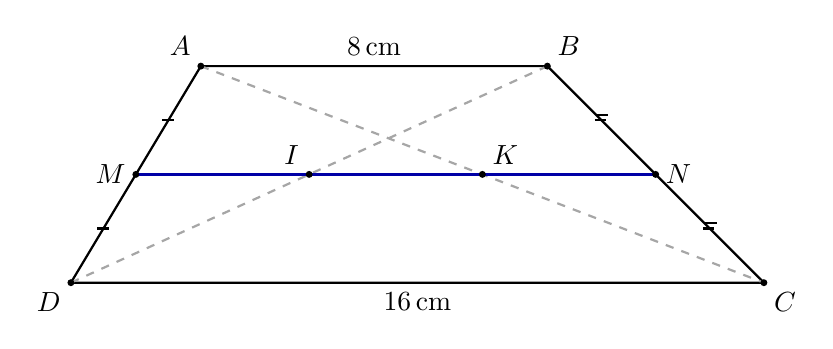
\begin{tikzpicture}[scale=0.55,thick]
\coordinate (A) at (3,5);
\coordinate (B) at (11,5);
\coordinate (C) at (16,0);
\coordinate (D) at (0,0);
\coordinate (M) at ($(A)!0.5!(D)$);
\coordinate (N) at ($(B)!0.5!(C)$);
\coordinate (I) at (intersection of M--N and B--D);
\coordinate (K) at (intersection of M--N and A--C);
\draw (A)--(B)--(C)--(D)--cycle;
\draw[dashed,gray!70] (A)--(C) (B)--(D);
\draw[blue!65!black] (M)--(N);
\draw ($(A)!0.25!(D)+(-0.14,0)$)--($(A)!0.25!(D)+(0.14,0)$);
\draw ($(A)!0.75!(D)+(-0.14,0)$)--($(A)!0.75!(D)+(0.14,0)$);
\draw ($(B)!0.25!(C)+(-0.16,0)$)--($(B)!0.25!(C)+(0.10,0)$);
\draw ($(B)!0.25!(C)+(-0.10,0.12)$)--($(B)!0.25!(C)+(0.16,0.12)$);
\draw ($(B)!0.75!(C)+(-0.16,0)$)--($(B)!0.75!(C)+(0.10,0)$);
\draw ($(B)!0.75!(C)+(-0.10,0.12)$)--($(B)!0.75!(C)+(0.16,0.12)$);
\filldraw (A) circle (1.5pt) (B) circle (1.5pt) (C) circle (1.5pt) (D) circle (1.5pt) (M) circle (1.5pt) (N) circle (1.5pt) (I) circle (1.5pt) (K) circle (1.5pt);
\node[above left] at (A) {$A$};\node[above right] at (B) {$B$};
\node[below right] at (C) {$C$};\node[below left] at (D) {$D$};
\node[left] at (M) {$M$};\node[right] at (N) {$N$};
\node[above left] at (I) {$I$};\node[above right] at (K) {$K$};
\node[above] at ($(A)!0.5!(B)$) {$8\,\mathrm{cm}$};
\node[below] at ($(D)!0.5!(C)$) {$16\,\mathrm{cm}$};
\end{tikzpicture}
\end{document}
